\pagestyle{plain}
\chapter{Metodologia}



\section{Materiais e métodos}

\subsection{População e amostra}


A amostra populacional estratificada desta pesquisa será realizada de forma considerará a diversidade socioambiental e cultural do território de identidade e seus municípios (\ref{fig:1}).


\begin{figure}[H]
  \centering
  \caption{Quadrantes e categorias adotadas no posicionamento hierárquico de pontos}
  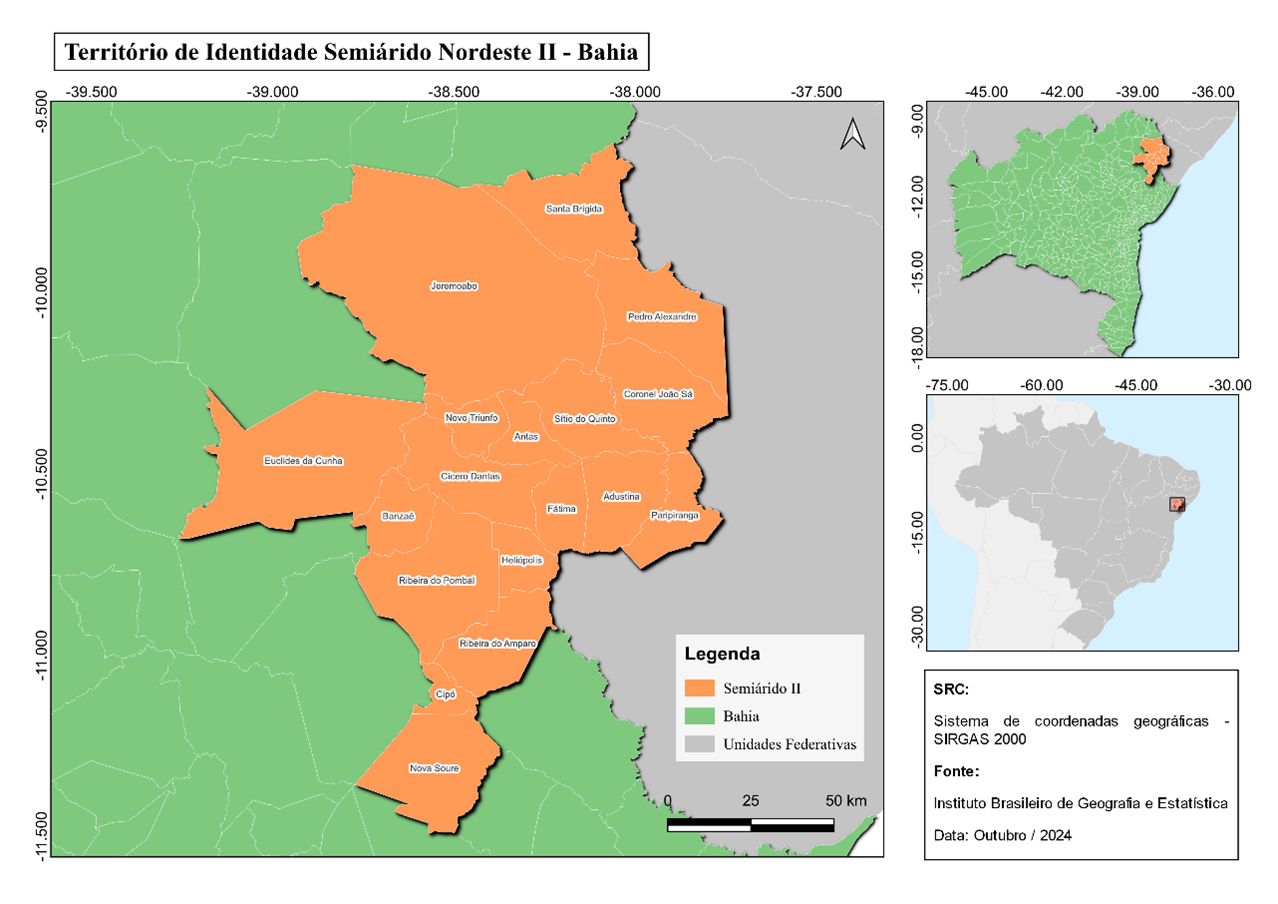
\includegraphics[scale=0.5]{Imagens/fig_1.png}
  \fonte{\textbf{Elaborado pelos autores} (2025)}
  \label{fig:1}
\end{figure}


Atualmente o total da população do território de identidade Semiárido Nordeste II é de 425.976 habitantes, tendo os municípios de: Adustina (17.209 hab.), Antas (19.659 hab.), Banzaê (13.251 hab.), Cícero Dantas (32.636 hab.), Cipó (17.402 hab.), Coronel João Sá (15.549 hab.), Euclides da Cunha (61.112 hab.), Fátima (17.801 hab.), Heliópolis (12.946 hab.), Jeremoabo (40.832 hab.), Nova Soure (24.236 hab.), Novo Triunfo (15.445 hab.), Paripiranga (29.124 hab.), Pedro Alexandre (16.698 hab.), Ribeira do Amparo (14.631 hab.), Ribeira do Pombal (54.097 hab.), Santa Brígida (13.917 hab.), Sítio do Quinto (9.431 hab.). Desta população foram selecionados os remanescentes registrados, que contam com a cidade de Jeremoabo sua maior representação. 
O município conta com as comunidades quilombolas de: Algodões, Algodões dos Negros, Angico, Ariade, Baixão da Tranqueira, Baixão da Viração, Casinhas, Olho D'Água, Olho D'Água dos Negros, Vasos do Ouricuri e Viração. Para a realização da pesquisa, serão adotados critérios de inclusão, os quais considerarão produtores agrícolas com idade igual ou superior a 18 anos, de ambos os sexos, residentes nas comunidades registradas no Base de Informações sobre os Povos Indígenas e Localidades Quilombolas do IBGE, (2019) que concordarem em participar do estudo.
A amostra populacional será calculada com base em uma margem de erro de 5,0\%, um nível de confiança de 95\% e uma proporção estimada de 50\% para as estimativas intervalares e uma proporção estimada de $\pi=0,5$ para as proporções de interesse, segundo a fórmula 1.

%% colocar a fórmula

A coleta de dados será realizada por uma equipe de entrevistadores previamente selecionados e treinados. Eles seguirão um manual de orientação para a realização das entrevistas, preenchimento dos instrumentos e relatórios, além de receberem supervisão e orientações sistemáticas durante todo o processo. O processo da pesquisa pode ser compreendido a partir do fluxograma descrito na Figura 2.


\begin{figure}[H]
  \centering
  \caption{Quadrantes e categorias adotadas no posicionamento hierárquico de pontos}
  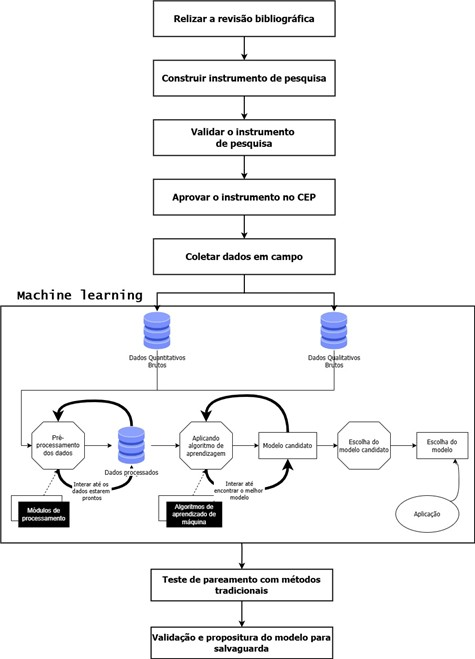
\includegraphics[scale=0.5]{Imagens/fig_2.jpg}
  \fonte{\textbf{Elaborado pelos autores} (2025)}
  \label{fig:2}
\end{figure}


\subsubsection{Dimensões analisadas}

O primeiro construto será composto por itens que compreenderão a percepção dos conhecimentos etnoclimatológicos, etnopedológicos e etnoecológicos. Tais conhecimentos constituem elementos fundamentais do repertório dos saberes tradicionais. Os conhecimentos etnoclimatológicos se referem à profunda compreensão que comunidades tradicionais detêm acerca das características climáticas específicas de suas regiões, abrangendo a identificação precisa de padrões de precipitação, ventos, e as flutuações sazonais correspondentes (Padigala, 2015).
Paralelamente, os conhecimentos etnopedológicos englobam a apreensão e aplicação de informações concernentes às propriedades e categorias de solos regionais, contemplando a análise da fertilidade do solo, sua composição e a determinação de usos agrícolas adequados (Barrera-Bassols; Alfred Zinck; Van Ranst, 2006). Ademais, os conhecimentos etnoecológicos compreende o conhecimento ecológico e ambiental de base cultural, a percepção cultural e a cognição do mundo natural e os comportamentos e práticas associados (Pieroni; Price; Vandebroek, 2005).

O segundo construto será avaliado a partir da percepção do valor do conhecimento tradicional. Esta dimensão será composta por questões, como a compreensão da percepção do valor do conhecimento tradicional que é fundamental para o entendimento da visão dos povos e comunidades tradicionais quanto à valorização de suas práticas e saberes agrícolas acumulados ao longo de gerações (Lakshmanan; Lakshmanan, 2014). Esses conhecimentos, muitas vezes passados oralmente de geração em geração, representando uma rica fonte de informações sobre o meio ambiente e as melhores formas de interação, porém não conhecidamente valorizados.

O terceiro construto compreenderá a capacidade de adaptação às mudanças ambientais. Essa dimensão será composta por itens que buscará compreender a capacidade dos povos e comunidades estudadas à adaptação de mudanças. Essa adaptação é evidenciada pelo modo como essas comunidades modificam suas práticas e conhecimentos agroecológicos em resposta a variações no clima, na biodiversidade ou em outros aspectos de seus ambientes naturais, surgindo assim inovações e tecnologias (Zhong et al., 2022). 
Por exemplo, mudanças nos padrões de precipitação podem levar às alterações nas práticas agroecológicas, como a escolha de culturas resistentes à seca ou a alteração do calendário de plantio e colheita (Verma, 2019). Essas adaptações são fundamentadas em um profundo entendimento do meio ambiente local e na experiência acumulada ao longo do tempo, permitindo que as comunidades mantenham sua sustentabilidade e modo de vida (Kline; Waring; Salerno, 2018).

O quarto construto compreenderá a análise da originalidade do conhecimento tradicional. Essa dimensão será analisada a partir de resultados de itens, como a originalidade do conhecimento tradicional que é evidenciada na forma como essas comunidades interpretam e interagem com o mundo natural (Kawecki; Ebert, 2004).
Este conhecimento não é apenas uma acumulação de fatos ou práticas, ele é enriquecido por perspectivas culturais, históricas e espirituais que conferem uma profundidade e uma complexidade que vão além do entendimento superficial do meio ambiente (D’Ambrosio, 2015). Por exemplo, práticas agrícolas tradicionais podem não ser apenas métodos de cultivo, mas também inclusão de rituais e crenças que refletem a relação espiritual da comunidade com a terra (Souravi; Rajasekharan, 2019).

E por fim, o quinto construto será analisado a partir da compreensão das práticas agroecológicas tradicionais comunitárias. O construto será composto por questões, que buscam representar um conjunto de métodos e saberes agrícolas que são desenvolvidos, mantidos e transmitidos dentro de comunidades tradicionais (Altieri, 2019). Essas práticas são caracterizadas por uma profunda compreensão e respeito pelo equilíbrio natural na produção agrícola e agroflorestal, enfatizando a sustentabilidade, a biodiversidade e a harmonia com o meio ambiente (Irhza et al., 2023).


\subsubsection{Operacionalização de Variáveis}

A construção de conhecimentos e saberes tradicionais abrangem diversos construtos que um bem imaterial pode possuir, gerenciar e controlar. Essas dimensões variam conforme as diferentes estruturas conceituais adotadas. Portanto, esta pesquisa será baseada em um referencial teórico que delineia as percepções dos saberes tradicionais, incluindo os seguintes aspectos do conhecimento: etnoclimatológicos, etnopedológicos, etnoecológicos (Borah; Ladon; Garkoti, 2023; Fernández-Llamazares et al., 2015; Nazarea, 2006) ; percepção do valor do conhecimento tradicional (Gavin et al., 2015), adaptação às mudanças ambientais (Fernández‐Llamazares; Cabeza, 2018), originalidade do conhecimento tradicional e práticas agroecológicas tradicionais comunitárias (Altieri, 2002).


\subsubsection*{Análise dos dados textuais selecionados}

\subsubsection*{\textit{Análise quantitativa dos dados textuais}}

Após a seleção dos comentários diretamente relacionados ao tema proposto nesta pesquisa, foram realizadas lexicométricas e análises de discursos nos textos presentes com o auxílio do software IRaMuTeQ \cite{Paulovich2008,DaSilvaCezar2018}. Através da utilização de Unidades de Contexto Iniciais (UCIs) na construção do modelo para análise, foi realizada uma prévia correção no conjunto de dados brutos, mantendo as palavras analisáveis, os termos caracterizados como substantivos, adjetivos e verbos. As palavras que geralmente não são relevantes para uma análise, como preposições e advérbios, foram excluídas.

Ao se trabalhar com corpus textuais, cada conjunto de texto deve compor uma UCI. Um conjunto de UCI é conhecido como corpus de análise, que o software segmenta em textos de aproximadamente três linhas, chamados Segmentos de Texto (ST) \cite{Fernandes2018ManualPortuges}. 

\subsubsection*{\textit{Análise qualitativa dos dados}}

Após a segmentação dos textos, foi realizada uma Classificação Hierárquica Descendente (CHD) dando origem a classes lexicais caracterizadas pelo vocabulário e a segmentos de textos que partilham o mesmo vocábulo. A CHD consiste em uma categoria de análise de conglomerado que categoriza as palavras obtidas em classes lexicais (eixos). A análise avalia a constância e os arranjos das palavras ativas no \textit{corpus} textual usando os dados das tabelas de contingência das palavras existentes \cite{Mendes2019,Carvalho2020a}. 

Neste sentido, as diferentes classes resultantes representam o espaço de sentido das palavras narradas, surgindo, assim, elementos pertencentes aos temas observáveis da pesquisa \cite{Gavasso2016}.


\subsection{Construção do instrumento de pesquisa}

O instrumento de pesquisa será estruturado em duas partes. A primeira parte compreenderá questões sociodemográficas, como idade, gênero, nível educacional, ocupação, tempo de residência na comunidade e envolvimento em atividades agrícolas. A segunda parte do instrumento será composta por perguntas fechadas e abertas que abordarão os cinco construtos principais: conhecimentos etnoclimatológicos, etnopedológicos e etnoecológicos; percepção do valor do conhecimento tradicional; capacidade de adaptação às mudanças ambientais; originalidade do conhecimento tradicional; e práticas agroecológicas tradicionais comunitárias. Cada construto será avaliado por meio de uma série de itens específicos, totalizando aproximadamente 25 a 30 perguntas. As perguntas serão formuladas de maneira clara e objetiva, utilizando uma linguagem acessível para garantir a compreensão por parte dos participantes. A escala de resposta para as perguntas fechadas será do tipo Likert, variando de "discordo totalmente" a "concordo totalmente", permitindo a quantificação das percepções dos participantes. As perguntas abertas permitirão aos participantes expressar suas opiniões e experiências de forma mais detalhada, proporcionando uma compreensão mais profunda dos temas abordados.

\subsubsection*{\textit{Protocolo de validação dos instrumentos}}

Após a formulação e estruturação dos itens a serem utilizados no instrumento de coleta de dados, este foi submetido à validação com base no modelo tripartite, descrito no \textit{Standards for Educational and Psychological Testing} \cite{Association2018}, que apresenta o processo de validação nas seguintes fases: 

\begin{enumerate}
\item Validação de conteúdo; 
\item Validade baseada na estrutura interna; 
\item Validade baseada nas relações com medidas externas; 
\item Validade baseada no padrão de resposta aos itens e
\item Validade consequencial.
\end{enumerate}

\subsubsection*{\textit{Validade de conteúdo}}

Para medir a eficácia do questionário proposto neste estudo, o método Coeficiente de Validade de Conteúdo (CVC) foi utilizado como parâmetro de verificação. Essa técnica envolve a busca do bom senso de uma comunidade de juízes (ou seja, profissionais efetivamente envolvidos na área de pesquisa). O método CVC baseia-se na aplicação estruturada do conhecimento e da experiência de especialistas da área, pressupondo que o julgamento conjunto de um determinado processo, se bem organizado, é melhor que a opinião de uma única pessoa \cite{Santos2018,Gurgel2021}.

O CVC é uma técnica quantitativa em que se calcula a concordância que juízes distintos possuem sobre um mesmo instrumento. Habitualmente, isso é feito solicitando que eles atribuam um valor gradual (1 a 5) aos itens, em função da clareza da linguagem de cada item (a quão clara e compreensível está a sentença), pertinência (o quanto o item é pertinente para analisar a dimensão analisada) e relevância (o quanto ele pode discriminar o construto e o quanto é relevante para a medida).  Após isso, basta aplicar a equação \ref{eq:1}:

\begin{equation}
CVC_{i}=\frac{k}{j}*\left (\frac{\sum_{i}=1x_{i}}{E}\right)
\label{eq:1}
\end{equation}

Em que: (K) é o número de itens; (Xi) é cada item; (J) é o número de juízes; (E) é o número de itens da escala (questionário).

De modo que o resultado de CVC foi obtido pela Equação \ref{eq:2}:

\begin{equation}
CVC=\frac{1}{N}*CVC_{i}
\label{eq:2} 
\end{equation}

Onde: (N) é o número de itens.

Por fim, foi solicitado a cada juiz se houve necessidades de modificação do item. A avaliação do questionário pelos juízes foi realizada às cegas, portanto, acreditou-se que a confidencialidade dos participantes garantiu maior fidelidade aos resultados ao final do experimento e permite uma melhor exposição, além de manter a sua compreensão do questionário proposto \cite{Hasson2000}.

\subsubsection*{\textit{Validade baseada na estrutura interna}}

\begin{enumerate}
\item Invariância Configural;
\item Invariância Métrica; 
\item Invariância Escalar.
\end{enumerate}


\citeonline{Borsa2018} explica que a Invariância Configural é um método utilizado para avaliar o grau de equivalência da estrutura fatorial da ferramenta para grupos diferentes (testa se a distribuição dos itens por fator ainda é suficientemente aceitável para amostras diferentes).

A invariância métrica avalia se as cargas fatoriais dos itens para grupos diferentes se mantêm, em outras palavras, avalia o grau em que os itens têm a mesma importância para a avaliação de estruturas em amostras diferentes. 

Por fim, a Invariância Escalar verifica se as pontuações obtidas estão totalmente relacionadas com o nível de traço latente dos sujeitos, independentemente do grupo a que pertençam, este teste é realizado estipulando que os interceptos dos itens para os diferentes grupos são iguais.

Para avaliar a invariância do questionário, foram utilizados os testes de diferença do \textit{Comparative Fit Index} ($\triangle$CFI) e a diferença por qui-quadrado. Para assumir a invariância da medida, em comparação com o modelo anterior, o índice de ajuste do modelo de teste no CFI não deve ser maior que 0.01 \cite{Cheung2002EvaluatingInvariance}, e para o valor do $\delta\chi^2$  deve apresentar um valor de p> 0.05 \cite{Milfont2010TestingResearch.}.

\subsubsection*{\textit{Validade de Critério Discriminante}}

\subsubsection*{\textit{Validade consequencial}}

O método de validade baseado em argumentação da consequência envolve exposição explicativa dos conteúdos e argumentação da validade inerente à hipótese buscada pela ferramenta, \cite{Kane2010}. O argumento explicativo especifica a interpretação proposta e o uso dos resultados do teste e estabelece uma rede de inferências e hipóteses a partir do desempenho observado até as conclusões e decisões baseadas no desempenho, \citeonline{Lane2014ValidityConsequences}

Este trabalho adotou como método de validação consequencial o delineamento adaptado de \citeonline{Zhang_J}:

\begin{enumerate}[label=\roman*]

\item Relatar os efeitos pretendidos do sistema de avaliação.
\item Descrever os componentes do sistema de avaliação, além de um fundamento lógico e coerente para cada componente, incluindo o apoio para esse fundamento teórico.
\item As afirmações interpretativas feitas a partir dos resultados da avaliação.
\item Os mecanismos de ação designados para causar os efeitos pretendidos.
\end{enumerate}

\subsubsection*{\textit{Validade baseada no padrão de resposta aos itens}}

Para validação baseada no padrão de respostas aos itens, esta validação foi adotada com os seguintes pressupostos:

\begin{enumerate}[label=\roman*.]
\item Itens claros não geram desinteresse no ato de responder;
\item Itens objetivos não geram respostas distantes do traço latente do avaliado;
\item Questionário objetivo não gera cansaço exagerado ao responder.
\end{enumerate}


\begin{enumerate}
\item ($H_1$) O Conhecimento Ecológico Tradicional (CET) tem um efeito positivo na validação de sistemas agroecológicos tradicionais;
\item ($H_2$) A Valorização do Conhecimento Tradicional (VCT) tem um efeito positivo na conservação de práticas agroecológicas sustentáveis e
\item ($H_3$) A Organização do Conhecimento Tradicional (OCT) tem um efeito positivo na transmissão intergeracional de saberes agroecológicos.
\end{enumerate}


\begin{figure}[H]
  \centering
  \caption{Rede nomológica de relacionamentos conceituais da percepção estudada}
  
\includegraphics[scale=0.7]{Imagens/fig_14.pdf}
  \fonte{\textbf{Elaborado pelos autores} (2022)}
  \label{fig:17}
\end{figure}





\subsubsection*{\textit{Análise por Modelagem por equações estruturais}}

Buscando compreender melhor as interações dos construtos e as variáveis preditivas do questionário, uma modelagem de equação estrutural de mediação múltipla foi implementada a partir dos dados apresentados pelos detentores de conhecimento tradicional para identificar quais os valores atribuídos aos saberes agroecológicos tradicionais das comunidades quilombolas do semiárido baiano influenciam a validação e preservação desses conhecimentos. A Modelagem de Equação Estrutural (MEE) refere-se a um conjunto de equações com os pressupostos do sistema analisado, onde os parâmetros são determinados com base na observação estatística. Assim, as equações estruturais referem-se a equações que usam parâmetros na análise das variáveis observáveis ou latentes, objetivando determinar o grau em que uma modelo empírico proposto é suportado pelos dados \cite{Tarka2018AnSciences}.

A MEE se mostra muito versátil, e as aplicações aumentando desde os primórdios  reconstruídos indiretamente com base nos trabalhos de Spearman (\citeyear{spearman_C_1904,Spearman_1927}). O que diferencia a MEE de outras ferramentas estatísticas são as combinações entre análise fatorial e análise de caminho, podendo medir e acomodar erros das variáveis observadas, extrair fatores por várias variáveis observáveis e estimar as relações entre estes \cite{Xiong2016}. Usualmente, essa abordagem é composta por um modelo de medida e um modelo estrutural. Para este estudo foram tomados como dados pressupostos de relação, as relações existentes entre os construtos relatados na literatura.

Os dados da escala foram inicialmente avaliados quanto à normalidade usando o teste de Kolmogorov-Smirnov [K-S = 0.242, p < 0.000]. Como os dados não apresentavam distribuição normal, foi realizada a correlação de Spearman. Para esta análise acima, foi utilizado o \textit{Statistical Package for the Social Sciences} SPSS, versão 25.0 \cite{SPSSCorp2017}.

Um modelo de segunda ordem foi proposto utilizando a Análise Fatorial Confirmatória, diferente da AFE ela tem uma estrutura predeterminada, ou seja, o pesquisador determina a que fator pertence cada variável, de modo a confirmar se as variáveis observadas conseguem  representar os fatores. No modelo estrutural são definidas as relações causais ou de associação hipotéticas entre as variáveis latentes, especificando se uma variável latente causa mudanças, direta ou indiretamente, em outras variáveis latentes.

As variáveis, sejam elas observadas ou latentes, podem ser classificadas em exógenas (independentes ou preditoras), quando não sofrem efeito de nenhuma outra variável no modelo, ou endógenas (dependentes), quando são influenciadas por outras variáveis e é sempre acompanhada de um termo residual, ou seja, \cite{Iacobucci2010StructuralTopics}. Dessa forma, é importante que o pesquisador tenha conhecimento a respeito do tema investigado, de modo a determinar corretamente quais variáveis são as independentes (preditoras) e quais são dependentes (consequência) no modelo a ser testado. 

O termo residual, ou de erro, junto ao erro de mensuração, representam as causas omitidas das variáveis endógenas, podendo estar associado a variáveis observadas ou latentes. Quando associado à variável observada, diz respeito à variação não explicada pela variável latente que a variável correspondente deve medir, ou por qualquer outra variável latente. Associado a uma variável latente, representa a variação nessa variável, não atribuída aos indicadores que a definem, e sim a todas as outras não observáveis \cite{Iacobucci2009EverythingAsk}.

Inicialmente, para implementação da MEE, é definido um modelo que evidencia as relações hipotéticas entre o conjunto de variáveis analisadas, decorrente da obtenção de relações empíricas resultantes da AFE. Para representar tais relações é comumente utilizado um esquema visual denominado Diagrama de Caminhos.

A modelagem de equações estruturais foi implementada  utilizando o software R Studio, por meio do método dos \textit{Weighted Least Squares Mean and Variance Adjusted} (WLSMV) similar ao RDWLS (utilizada quando as variáveis são dicotómicas) e útil para dados categóricos presentes em matrizes policóricas não normalmente distribuídas. Os efeitos de mediação foram obtidos pela técnica de bootstrapping com 5.000 reamostragens para um intervalo de confiança de 95\% do efeito mediado. Para avaliar o modelo global, foram considerados os mesmos índices de ajuste utilizados na AFE (RMSEA, CFI e TLI), assim como o $X^2$ e $X^2$/df.

A acurácia preditiva dos construtos foi avaliada pelo coeficiente de determinação ($R^2$). Segundo \citeonline{HairJr2021APLS-SEM}, nas pesquisas que se baseiam na validação de conhecimentos tradicionais, um intervalo de $R_2$ entre 0.75 e 0.50 podem ser considerados substancial a moderado, respectivamente.

\subsubsection*{\textit{Análise dos itens por Modelo Rasch}}

Os itens foram analisados usando a teoria de resposta ao item por dois parâmetros logísticos \cite{Andrich1978ACategories}. A análise de Rasch para compreender as dificuldades dos itens politômicos formadores do modelo foi realizada para determinar quais as relevâncias e cargas das questões que validaram as hipóteses aceitas no modelo.

Para verificar a segurança do instrumento e possíveis desvios no desempenho não esperados, foram avaliados indicadores de \textit{Infit} e \textit{Outfit} tanto para pessoas quanto para os itens. Em relação aos índices de fidedignidade, são esperados valores maiores que 0.70 ou, preferencialmente, valores maiores que 0.80 \cite{Linacre2012WinstepsGuide}.

O \textit{Infit} avalia padrões de resposta inesperados de indivíduos que apresentam um nível de traço latente ($\theta$) equivalente ao nível de dificuldade do item. Outfit, no que lhe concerne, verifica padrões de resposta inesperados daqueles que apresentam um nível de theta - $\theta$ abaixo ou acima do nível de dificuldade do item. As estimativas de \textit{Infit} e \textit{Outfit} podem ser avaliadas pelos indicadores quadrado médio (\textit{mean square}; MNSQ) e z-padronizado (z standardized; ZSTD). 

Para o MSNQ, o valor padrão esperado é 1. Valores maiores que 1 indicam que as estimativas apresentaram mais variação do que o esperado pelo modelo Rasch (ou seja, desajuste) enquanto valores menores que 1 indicam menos variação do que o esperado pelo Modelo Rasch (ou seja, sobreajuste). As pontuações aceitáveis do MNSQ normalmente variam de 0.7 a 1.3 logits \cite{Boone2016RaschHow,Bond2020ApplyingSciences}, mas um intervalo menos conservador de 0.5-1.5 \textit{logits} também pode ser usado \cite{Wright1994ReasonableTransactions}. Já para o ZSTD, valores acima de |2| indicam que a estimativa não se ajusta adequadamente aos dados.

O DIF foi avaliado por meio do procedimento de Mantel \cite{Bond2020ApplyingSciences}. Itens cujas estimativas de dificuldades se apresentaram como estatisticamente diferentes para homens e para mulheres (p $\leq$ 0.05) foram inspecionados. A magnitude do DIF foi interpretada através do DIF contrast: valores entre | 0.00 | e | 0.43 | são considerados baixos; valores entre | 0.44 | e | 0.64 | são considerados moderados; e valores acima de | 0.64 | são considerados altos. As análises foram desenvolvidas utilizando o software Winsteps versão 5.1.4 \cite{Linacre2012WinstepsGuide}.



\subsubsection*{\textit{Medidas utilizadas}}


\begin{figure}[H]
  \centering
  \caption{Modelo configuracional}
  
\includegraphics[scale=0.3]{Imagens/fig_18.pdf}
  \fonte{\textbf{Elaborado pelos autores} (2022)}
  \label{fig:18}
  \footnotesize{Nota: Conhecimento Ecológico Tradicional (CET), Valorização do Conhecimento Tradicional (VCT), Contextualização Ambiental (CAM), Organização do Conhecimento Tradicional (OCT), Práticas Agroecológicas Tradicionais (PAT), Agentes e comunidades detentoras de conhecimento (ACT), Transmissão e documentação de saberes tradicionais (TDS), Disponibilidade de recursos e biodiversidade local (DRB), Sistemas Agroecológicos Tradicionais (SAT) e Validação de práticas sustentáveis tradicionais (VPS)}
\end{figure}


\subsubsection*{\textit{Análise de dados e descobertas por fsQCA}}

A fim de compreender quais as condições suficientes e necessárias para construção de um modelo empírico de validação de saberes tradicionais agroecológicos, neste estudo, nove construtos (variáveis constituintes) foram considerados variáveis de condição para análise de comparação usando fsQCA para investigar o efeito dos conhecimentos tradicionais quilombolas na validação e preservação de sistemas agroecológicos sustentáveis do semiárido baiano.


\subsubsection*{Teoria fundamentada em dados — sub-escala CTA-Semiárido}

Medição de pontos:
\begin{enumerate}
\item Não se aplica;
\item Usualmente não se aplica;
\item Ocasionalmente se aplica;
\item Usualmente se aplica;
\item Sempre se aplica.
\end{enumerate}

A Tabela \ref{tab:15} descreve os códigos e indicadores formadores dos \textit{clusters} utilizados.

\newpage
\begin{landscape}
\begin{longtable}{@{}lcp{4cm}p{9cm}@{}}
\caption{Códigos e guias de consulta para conhecimentos agroecológicos tradicionais}\label{tab:15}\\
\toprule
 &
  \textbf{Iniciais} &
  \textbf{Código} &
  \textbf{Descrição} \\ \midrule
\endfirsthead
%
\multicolumn{4}{c}{{\tablename\ \thetable{} -- continuação da página anterior}} \\
\toprule
 &
  \textbf{Iniciais} &
  \textbf{Código} &
  \textbf{Descrição} \\ \midrule
\endhead
%
\midrule
\multicolumn{4}{r}{{Continua na próxima página}} \\
\endfoot
%
\bottomrule
\endlastfoot
%
\multirow{4}{*}{\textbf{\rotatebox{90}{\textit{CLUSTER} 1}}} &
  1A &
  Identificando os detentores do conhecimento &
  O código refere-se aos agentes detentores dos conhecimentos agroecológicos tradicionais nas comunidades quilombolas, incluindo agricultores, anciãos e lideranças comunitárias. \\
 &
  1B &
  Compreendendo as estruturas comunitárias &
  O código abrange as formas de organização social e transmissão dos saberes dentro das comunidades tradicionais do semiárido baiano. \\
 &
  1C &
  Mapeando redes de conhecimento &
  O código objetiva identificar as conexões e intercâmbios de saberes entre diferentes comunidades e agentes externos (universidades, ONGs, governo). \\
 &
  1D &
  Avaliando impactos territoriais &
  O código visa compreender como os conhecimentos tradicionais influenciam a gestão territorial e a conservação dos recursos naturais locais. \\
\multirow{4}{*}{\textbf{\rotatebox{90}{CLUSTER 2}}} &
  2A &
  Catalogando práticas etnoclimatológicas &
  Sobre os conhecimentos relacionados aos padrões climáticos, previsão do tempo e adaptação às variações sazonais no semiárido. \\
 &
  2B &
  Documentando saberes etnopedológicos &
  Sobre os conhecimentos tradicionais relacionados aos tipos de solo, fertilidade, manejo e conservação das propriedades edáficas. \\
 &
  2C &
  Registrando conhecimentos etnoecológicos &
  O código visa capturar os saberes sobre interações ecológicas, biodiversidade local e manejo de ecossistemas nativos. \\
 &
  2D &
  Sistematizando práticas agroecológicas &
  O código abrange as técnicas tradicionais de cultivo, rotação, consórcio, manejo de pragas e doenças de forma sustentável. \\
\multirow{4}{*}{\textbf{\rotatebox{90}{CLUSTER 3}}} &
  3A &
  Avaliando processos de transmissão &
  Visa compreender como os conhecimentos são passados entre gerações e quais fatores facilitam ou dificultam essa transmissão. \\
 &
  3B &
  Analisando mecanismos de validação &
  Sobre como as comunidades validam, testam e adaptam seus conhecimentos tradicionais ao longo do tempo. \\
 &
  3C &
  Identificando ameaças aos saberes &
  Sobre quais fatores (modernização, êxodo rural, mudanças climáticas) ameaçam a continuidade dos conhecimentos tradicionais. \\
 &
  3D &
  Mapeando estratégias de resistência &
  Visa compreender como as comunidades mantêm e fortalecem seus saberes diante das pressões externas e mudanças socioambientais. \\
\multirow{4}{*}{\textbf{\rotatebox{90}{CLUSTER 4}}} &
  4A &
  Desenvolvendo protocolos de registro &
  O código refere-se às metodologias para documentação e sistematização participativa dos conhecimentos agroecológicos tradicionais. \\
 &
  4B &
  Implementando tecnologias de mapeamento &
  Sobre a aplicação de machine learning e outras tecnologias digitais para o mapeamento e validação dos saberes tradicionais. \\
 &
  4C &
  Criando sistemas de salvaguarda &
  Sobre o desenvolvimento de mecanismos legais e institucionais para proteção e reconhecimento dos conhecimentos tradicionais. \\
 &
  4D &
  Promovendo diálogos interculturais &
  Visa estabelecer pontes entre conhecimento científico e tradicional, promovendo reconhecimento mútuo e colaboração. \\
\multirow{3}{*}{\textbf{\rotatebox{90}{CLUSTER 5}}} &
  5A &
  Fortalecendo identidades culturais &
  O código refere-se ao papel dos conhecimentos tradicionais na manutenção da identidade cultural e coesão social das comunidades. \\
  &
  5B &
  Promovendo desenvolvimento sustentável &
  Sobre como os saberes tradicionais contribuem para estratégias de desenvolvimento rural sustentável e conservação ambiental. \\
  &
  5C &
  Construindo patrimônio imaterial &
  O código visa a compreensão dos conhecimentos agroecológicos como patrimônio cultural imaterial e sua importância para as gerações futuras. \\* \bottomrule
\end{longtable}
\end{landscape}


\subsection{Metodologia Integrada para Identificação}

A presente pesquisa adota uma abordagem metodológica mista, fundamentada na integração entre métodos qualitativos participativos e técnicas quantitativas baseadas em algoritmos de aprendizado de máquina. O objetivo é testar a hipótese de que modelos de aprendizado ensemble — especificamente Random Forest, Gradient Boosting e Support Vector Machines (SVM) — apresentam desempenho preditivo mais estável e preciso na identificação de conhecimentos aplicáveis a sistemas agroecológicos do que algoritmos individuais.

Inicialmente, a etapa de coleta de dados será realizada junto às comunidades quilombolas, indígenas e ribeirinhas do Território de Identidade Semiárido Nordeste II, na Bahia. Serão conduzidas oficinas participativas e entrevistas semiestruturadas com representantes comunitários, visando mapear práticas agrícolas tradicionais, registrar memórias sociais e identificar elementos centrais dos saberes agroecológicos locais. Os dados coletados incluirão transcrições textuais, registros audiovisuais e coordenadas geográficas, compondo uma base multimodal rica em conteúdo contextual e cultural.

Após a coleta, os dados textuais passarão por um processo de pré-processamento utilizando técnicas de Processamento de Linguagem Natural (PLN), incluindo remoção de stopwords, lematização e vetorização por meio de representações como TF-IDF, Word2Vec ou embeddings contextuais derivados de modelos como BERT. A partir dessas representações, serão extraídas variáveis linguísticas e semânticas associadas às práticas agroecológicas, tais como ciclos agrícolas, nomes de espécies nativas, saberes medicinais e técnicas de cultivo.

A etapa seguinte compreende a fusão dos dados textuais com informações geoespaciais e ambientais (clima, tipo de solo, topografia), permitindo a construção de uma base de dados integrada e multidimensional. Técnicas de engenharia de atributos serão utilizadas para a redução de dimensionalidade, quando necessário, por meio de métodos como Análise de Componentes Principais (PCA) ou Uniform Manifold Approximation and Projection (UMAP).

Para a modelagem preditiva, serão treinados e avaliados modelos de aprendizado de máquina com foco na comparação entre algoritmos individuais e métodos ensemble. Os modelos considerados incluirão Random Forest, Gradient Boosting (como XGBoost ou LightGBM), e Support Vector Machines (com diferentes funções de kernel), além de modelos simples como k-Nearest Neighbors (kNN), Regressão Logística e Árvores de Decisão básicas. Os objetivos da modelagem incluem a classificação supervisionada de narrativas segundo sua relevância agroecológica e a segmentação não supervisionada de práticas por meio de algoritmos de clustering como KMeans ou DBSCAN.

A avaliação dos modelos será conduzida por meio de métricas técnicas de desempenho, tais como acurácia, F1-score, AUC-ROC (para tarefas supervisionadas), bem como Silhouette Score e Davies-Bouldin Index (para clustering). Complementarmente, será realizada uma validação participativa dos resultados com as comunidades locais, garantindo que os padrões identificados tenham relevância social, cultural e ecológica. Essa validação ocorrerá por meio de reuniões devolutivas e construção conjunta de produtos de comunicação, como cartilhas ilustradas, mapas interativos e vídeos educativos.

Os resultados obtidos serão consolidados em um relatório técnico-científico e no "Livro de Registro dos Saberes Agroecológicos Tradicionais do Território de Identidade Semiárido Nordeste II", com vistas ao seu encaminhamento ao Instituto do Patrimônio Histórico e Artístico Nacional (IPHAN). Além disso, buscar-se-á a inclusão desses saberes no programa internacional "Sistemas Importantes do Patrimônio Agrícola Mundial" da FAO, ampliando o reconhecimento e a proteção global do patrimônio agroecológico da região.

Essa abordagem metodológica é justificada pelo potencial demonstrado dos modelos ensemble em aplicações agrícolas complexas, conforme evidenciado por Elhussiny et al. (2023), que identificaram desempenho superior do modelo XGB-RF em relação a Random Forest e XGBoost isoladamente na predição de padrões de irrigação em contextos semiáridos, alcançando coeficiente de determinação (R²) de 0.929, frente a 0.796 (RF) e 0.825 (XGB) (Elhussiny, 2023).






\subsection{Metodologia para Análise de Perfis de Especialização com Base em Variáveis Sociodemográficas}

Para testar a hipótese de que a Análise de Correspondência Múltipla (ACM) — combinada com Teoria de Resposta ao Item (TRI) — é capaz de revelar associações significativas entre variáveis sociodemográficas e domínios de conhecimento agroecológico, será adotada uma abordagem quantitativa estruturada, centrada na aplicação de métodos estatísticos multivariados. O objetivo é identificar perfis de especialização nas comunidades quilombolas com base nos padrões latentes de respostas associadas ao conhecimento agroecológico.

A coleta de dados será realizada por meio de questionários aplicados em campo, com estrutura semiestruturada, contemplando três blocos principais: (i) variáveis sociodemográficas (idade, gênero, escolaridade, função social na comunidade, tempo de residência e origem familiar); (ii) indicadores de acesso e prática em domínios agroecológicos (manejo da água, cultivo de variedades crioulas, práticas agroflorestais, saberes fitoterápicos, entre outros); e (iii) autoavaliação da frequência e relevância do uso desses saberes. Os dados serão codificados em formato categórico, adequado à aplicação da ACM.

A Análise de Correspondência Múltipla será utilizada como técnica exploratória para mapear a estrutura relacional entre as categorias das variáveis, permitindo identificar agrupamentos e dimensões latentes que organizam os perfis de conhecimento agroecológico nas comunidades. Essa análise revelará, por exemplo, se determinados domínios do saber estão mais fortemente associados a faixas etárias específicas, funções comunitárias ou níveis de escolarização.

Complementarmente, será aplicada a Teoria de Resposta ao Item (TRI), em especial modelos politômicos como o modelo de resposta gradual (GRM), para estimar a probabilidade de um indivíduo com certo "nível latente de conhecimento" manifestar domínio sobre determinados itens agroecológicos. Esse componente permitirá inferir perfis de especialização com base na proficiência individual em múltiplos domínios de saber. A TRI também contribui para controlar efeitos de viés de item e refinar a estrutura métrica da escala utilizada.

Os resultados das análises serão interpretados com base em mapas perceptuais e perfis latentes de conhecimento, auxiliando na identificação de clusters de especialização e possíveis lacunas de transmissão intergeracional dos saberes. A validação dos achados ocorrerá com participação comunitária, por meio de encontros devolutivos com representantes quilombolas, a fim de confrontar os padrões estatísticos com as percepções socioculturais locais sobre os modos de aprender e praticar a agroecologia.

Ao articular a ACM com a TRI em um mesmo modelo empírico, esta metodologia permite capturar tanto os padrões relacionais visíveis entre variáveis quanto as dimensões latentes de conhecimento, oferecendo uma ferramenta robusta para diagnosticar a diversidade interna de saberes agroecológicos nas comunidades e subsidiar estratégias de fortalecimento e salvaguarda desses patrimônios imateriais.



\subsection{Delineamento Experimental para Avaliação de Modelos CNN na Classificação de Saberes Agroecológicos}

Com o objetivo de testar a hipótese de que modelos baseados em redes neurais convolucionais (CNN) superam abordagens tradicionais como TF-IDF e bag-of-words (BoW) na tarefa de classificação automática de narrativas agroecológicas, propõe-se um experimento controlado com múltiplas configurações de modelos de aprendizado supervisionado.

A base de dados utilizada será construída a partir das transcrições textuais oriundas de entrevistas, oficinas participativas e registros narrativos colhidos junto às comunidades quilombolas, indígenas e ribeirinhas do Território de Identidade Semiárido Nordeste II. Esses documentos serão anotados manualmente com rótulos referentes a diferentes domínios de saber agroecológico, como manejo de água, cultivo de espécies nativas, práticas agroflorestais, uso medicinal de plantas e gestão de sementes crioulas. O corpus será segmentado em unidades textuais curtas, representativas e semanticamente coesas, resultando em um conjunto de dados anotados com no mínimo 500 entradas.

O experimento será dividido em duas frentes principais de modelagem. Na primeira, serão utilizadas representações vetoriais tradicionais — TF-IDF e BoW — em conjunto com algoritmos clássicos de classificação, como Regressão Logística, Naive Bayes e Support Vector Machines (SVM). Na segunda frente, será implementada uma arquitetura de CNN com embeddings pré-treinados (como Word2Vec ou GloVe), combinando camadas convolucionais unidimensionais e max-pooling, seguidas por camadas densas com ativação softmax para classificação multiclasse. O treinamento será realizado sobre uma divisão estratificada de dados (70\% treinamento, 15\% validação, 15\% teste), com replicação por validação cruzada (k-fold, k = 5) para avaliar estabilidade e generalização dos modelos.

A avaliação de desempenho incluirá métricas clássicas, como acurácia, F1-score macro e micro, AUC-ROC, além do tempo de treinamento e inferência. Será atribuído destaque especial à capacidade dos modelos em classificar corretamente classes minoritárias, com menor frequência no corpus, refletindo a sensibilidade a saberes menos difundidos, mas socialmente relevantes. Considerar-se-á como superior o modelo que apresentar incremento de ao menos 10\% no F1-score em relação aos métodos tradicionais, acompanhado de menor propensão ao sobreajuste e desempenho mais estável entre os folds de validação.

Os resultados quantitativos serão complementados por uma validação participativa com representantes das comunidades, mediante devolutiva dos rótulos preditos e avaliação qualitativa da coerência dos agrupamentos automatizados com os modos de organização e transmissão dos saberes locais. Tal etapa é fundamental para assegurar que o modelo reflita não apenas padrões estatísticos, mas também lógicas culturais e epistemologias situadas.

O delineamento proposto baseia-se em evidências recentes da literatura, nas quais modelos CNN aplicados à linguagem natural demonstraram desempenho significativamente superior frente a vetores TF-IDF e BoW em tarefas de classificação semântica, especialmente em textos com linguagem informal, ambígua ou culturalmente específica (Kamyab et al., 2021; Souza et al., 2022; Yeasmin et al., 2022). Dessa forma, o experimento contribui empiricamente para avaliar o potencial da aprendizagem profunda na sistematização e valorização dos conhecimentos agroecológicos tradicionais.


\subsection{Delineamento Experimental para Aplicação de Algoritmos de Otimização Multiobjetivo (NSGA-II e MOEA/D) na Valorização de Saberes Tradicionais}

Com o objetivo de testar a hipótese de que algoritmos de otimização multiobjetivo, como NSGA-II e MOEA/D, são capazes de equilibrar a preservação cultural e a aplicabilidade científica dos saberes agroecológicos tradicionais, propõe-se um experimento fundamentado na modelagem computacional de múltiplos critérios concorrentes. A abordagem busca identificar soluções que maximizem simultaneamente a integridade cultural dos saberes e seu potencial de sistematização e uso científico, respeitando os contextos socioculturais das comunidades envolvidas.

Inicialmente, será construída uma base de dados estruturada com registros de saberes agroecológicos coletados por meio de oficinas, entrevistas e processos participativos com comunidades quilombolas, indígenas e ribeirinhas. Cada registro será descrito a partir de dois conjuntos de variáveis: (i) indicadores de valor cultural, como grau de ancestralidade, exclusividade comunitária, vínculo com práticas rituais ou cosmologias locais; e (ii) indicadores de aplicabilidade científica, como grau de replicabilidade, potencial para experimentação, compatibilidade com princípios da agroecologia e aplicabilidade em políticas públicas.

A partir desses dados, será construída uma função de avaliação multiobjetivo onde cada saber ou prática será tratado como uma unidade de decisão. Os algoritmos NSGA-II (Non-dominated Sorting Genetic Algorithm II) e MOEA/D (Multi-Objective Evolutionary Algorithm based on Decomposition) serão empregados para gerar fronteiras de Pareto que representem diferentes compromissos entre os objetivos em conflito: preservar o significado cultural dos saberes e, ao mesmo tempo, facilitar sua validação, replicação e integração a modelos científicos agroecológicos.

A solução de Pareto resultante permitirá identificar clusters de saberes que representam diferentes perfis de equilíbrio — desde práticas altamente culturalizadas, mas com menor aplicabilidade científica direta, até saberes tecnicamente robustos e transferíveis, mas culturalmente mais neutros. Esses perfis serão interpretados em conjunto com lideranças e agentes comunitários, a fim de validar se os resultados computacionais refletem percepções internas de valor e reconhecimento.

Este experimento se inspira em estudos que aplicaram NSGA-II para adaptar técnicas tradicionais a cenários contemporâneos sem descaracterizá-las, como a adaptação climática de habitações vernaculares em Xinjiang, onde a otimização preservou técnicas construtivas tradicionais ao mesmo tempo em que maximizou conforto térmico e eficiência energética (Tuluxun et al., 2025) (Tuluxun, 2025)
. Assim, a metodologia proposta tem potencial de inovar ao integrar saberes tradicionais em processos de tomada de decisão científica sem os subordinar a lógicas puramente tecnocráticas, contribuindo para a salvaguarda ativa e funcional do patrimônio imaterial agroecológico.

\newpage